\documentclass[11pt]{article}

\usepackage{a4wide}
\usepackage[utf8]{inputenc}
\usepackage[T2A]{fontenc}
\usepackage[russian]{babel}
\usepackage{graphicx}
\usepackage{color}
\usepackage[left=2.5cm,right=2.5cm,
    top=2.5cm,bottom=2cm,bindingoffset=0cm]{geometry}
\usepackage {amsthm}
\usepackage {amsmath}
\usepackage{amssymb}
\usepackage{pb-diagram}
\usepackage{placeins}

\newtheorem{Def}{Определение}
\newtheorem{statement}{Утверждение}
\newtheorem{theorem}{Теорема}
\newtheorem{lemma}{Лемма}
\newtheorem{Remark_s}{Замечание}[statement]
\newtheorem{Remark}{Замечание}
\theoremstyle{definition}
\newtheorem{Remark_l}{Замечание}[lemma]
\newenvironment{Proof}
{\par\noindent{\bf Доказательство.\\}} 
{\begin{flushright}$\Box$\end{flushright}}

\definecolor{gray}{rgb}{0.5,0.5,0.5}

\newcommand\Set[2]{\left\{ #1 \colon #2 \right\}}
\newcommand\Ref[1]{(\ref{#1})}
\newcommand\ftw[2]{\overline{#1,#2}}
\newcommand\RS{\Ref{system} }
\newcommand\beq{\begin{equation}}
\newcommand\eeq{\end{equation}}
\newcommand\dd[2]{\frac{\partial#1}{\partial#2}}

\begin{document}

\begin{titlepage}
\begin{center}
\includegraphics[width=8cm, height=4cm]{MSU}
\end{center}
\begin{center}
Московский государственный университет имени М.В. Ломоносова\\
\vspace{0.1 cm}
Факультет вычислительной математики и кибернетики\\
\vspace{0.1 cm}
Кафедра системного анализа

\vspace{3cm}
{\Large Морозова Татьяна Евгеньевна }\\
\vspace{1cm}

{\bf\LARGE Управление в моделях межвидового взаимодействия}\\ \vspace{2cm}
ВЫПУСКНАЯ КВАЛИФИКАЦИОННАЯ РАБОТА

\end{center}
\vspace{2cm}
\begin{flushright}

{\bf Научный руководитель:}\\
к.ф.-м.н., доцент\\ 
И.~В.~Рублев

\end{flushright}

 \vspace{4.5cm}

\centerline {Москва, 2018}

\end{titlepage}

\newpage
\tableofcontents
\newpage

%=============Введение============
\section{Введение}

Рассматривается модель пищевой цепи с управлением без внутривидовой конкуренции, состоящая из четырех звеньев и описываемая следующей системой:

\beq
\left\{
\begin{aligned}
\label{system}
	\dot x_1 &= x_1(r_1 + u_1- b_1x_2), \\
	\dot x_2 &= x_2(-r_2 - b_2x_3 + c_2x_1), \\
	\dot x_3 &= x_3(-r_3 + u_2 - b_3x_4 + c_3x_2), \\
	\dot x_4 &= x_4(-r_4 + c_4x_3).
\end{aligned}
\right.
\eeq

Здесь $x_i,\, i = \ftw{1}{4}$ --- численности популяций видов, $r_1 + u_1$ --- рождаемость первого вида,  $r_2, r_3-u_2, r_4$ --- смертности остальных видов, коэффициенты $b_1, b_2, b_3$ и $c_2, c_3, c_4$ отвечают за взаимодействие между популяциями. Все параметры строго положительны, а управления берутся из интервалов $U_1^* = [u_1^{min}, u_1^{max}], U_2^* = [u_2^{min}, u_2^{max}]$ соответственно. Управление можно интерпретировать как интенсивность отлова или <<подкармливания>> соответствующего вида в зависимости от знака.

Данная система обобщает модель хищника-жертвы, впервые введенную в работе \cite{Lotka}, описывающей кинетику химических реакций. В дальнейшем опубликовано большое количество работ, посвященных исследованию систем без управления: \cite{Murray}, \cite{Basykin}, \cite{three_spec}, \cite{darboux}, \cite{Bratus} и др. и лишь несколько посвященных системам с управлением. Двумерный случай с управлением первой координатой исследован в \cite{Ruble}, трехмерный частично изучен в \cite{Aushkap}. В данной работе рассматривается одна из моделей межвидового взаимодействия типа пищевая цепь. Исследование, проведенное в \cite{MathBio}, указывает на то, что системы четного и нечетного порядка подобного вида в отсутствии управления весьма сильно различаются по своим свойствам. А именно, в общем положении параметров модели (то есть исключая некоторые вырожденные случаи) лишь системы четного порядка имеют изолированные положения равновесия и являются биологически устойчивыми в том смысле, что ни у одного из видов численность не стремится к нулю, то есть все виды выживают. Поэтому весьма логичным представляется исследование именно четырехмерной пищевой цепи, как системы минимальной размерности, большей двух, обладающей свойством биологической устойчивости.

Управляющие параметры входят в показатели естественных роста и смертности первого и третьего вида, соответственно, так как это является обобщением двумерного случая: мы можем рассматривать четырехмерную систему, как две двумерные со введенной дополнительной связью между второй и третьей компонентой. В процессе исследования были предприняты попытки изучить систему с одним управлением, но объективные трудности привели к рассмотрению задачи именно с двумя управлениями как более простого варианта задачи на начальном этапе ее исследования.

Сложность исследования данной четырехмерной системы по сравнению с двумерной заключается в в трудности изучения поведения интегральных кривых, тогда как в модели хищник-жертва поведение траекторий полностью характеризуется первым интегралом. Вследствие этого возникает вопрос, как исследовать и решать задачу исходя лишь из свойств первого интеграла, найденного в работе \cite{MathBio}. Настоящая работа отвечает на этот вопрос и предлагает метод решения, исходящий из принципа уменьшения первого интеграла и построения соответствующих управлений.

Таким образом основной целью данной работы является исследование свойств рассматриваемой системы и синтез управления для задачи попадания в $\varepsilon$-окрестность множества положений равновесия за конечное время. Предложен и исследован метод приближения к положению равновесия и доказано, что предложенный синтез позволяет решить задачу за конечное время для любого начального положения системы.

%Данная система обобщает модель хищника-жертвы, впервые введенную в работе \cite{Lotka} описывающей кинетику химических реакций. В дальнейшем двумерные системы были исследованы в большом количестве работ, таких как \cite{Murray}, \cite{Basykin}. В статье \cite{Ruble} была полностью исследована двумерная система с управлением первой компонентой и доказано, что за конечное время можно привести ее в положение равновесия. 
%
%Также исследовались и трехмерные системы, например, в \cite{three_spec} и в \cite{darboux}.
%
%В общем случае исследовались и пищевые цепи произвольной длины, к примеру, в \cite{MathBio} был найден первый интеграл, который используется в настоящей работе.
%
%В данной работе основной целью является исследование свойств и синтеза управления для задачи попадания в $\varepsilon$-окрестность множества положений равновесия за конечное время. Был предложен и исследован метод приближения к положению равновесия и доказано, что для любого начального положения системы с помощью предложенного синтеза задачу можно решить за конечное время.

%=============Общие свойства===========
\section{Общие свойства системы}

\indent Из биологической интерпретации вытекает, что численность популяции не может быть отрицательной. В следующем утверждении будет показано, что система удовлетворяет этому свойству.

\begin{statement}
	Множество $\Set{x \in \mathbb{R}^4}{x_i > 0, i = \ftw{1}{4}}$ инвариантно относительно системы \RS.
\end{statement}
\begin{Proof}
	Из системы \RS видно, что при обнулении координат, обнуляются соответственно и выражения для $\dot x_i,$ так что координаты не могут поменять знак. Интегрируя в обратном времени, получим, что координаты не могут обнулиться.
\end{Proof}

Рассмотрим положения равновесия \RS как функцию управления: 
\begin{gather}
	P(u) = (P_1(u), P_2(u), P_3(u), P_4(u)),\; \text{где} \notag \\
	P_1(u) = \frac{r_2c_4 + b_2r_4}{c_2c_4}, \;\; P_2(u) = \frac{r_1 + u_1}{b_1}, \;\; P_3(u) = \frac{r_4}{c_4},\;\; P_4(u) = \frac{c_3(r_1+u_1) + (u_2 - r_3)b_1}{b_1b_3}.
\end{gather}

Заметим, что от управления существенно зависят только вторая и четвертая координата, поэтому в дальнейшем будем обозначать $P(u) = (P_1, P_2(u), P_3, P_4(u)).$ \\

Множество положений равновесия $\bar P = \Set{P(u)}{u \in U^*}$ представляет из себя параллелограмм в пространстве $(x_2, x_4).$ В нашей работе мы предполагаем его непустоту, для этого введем ограничение на параметры задачи:
$$P_4(u_1^{min}, u_2^{min}) > 0.$$

\begin{figure}[h]
\center{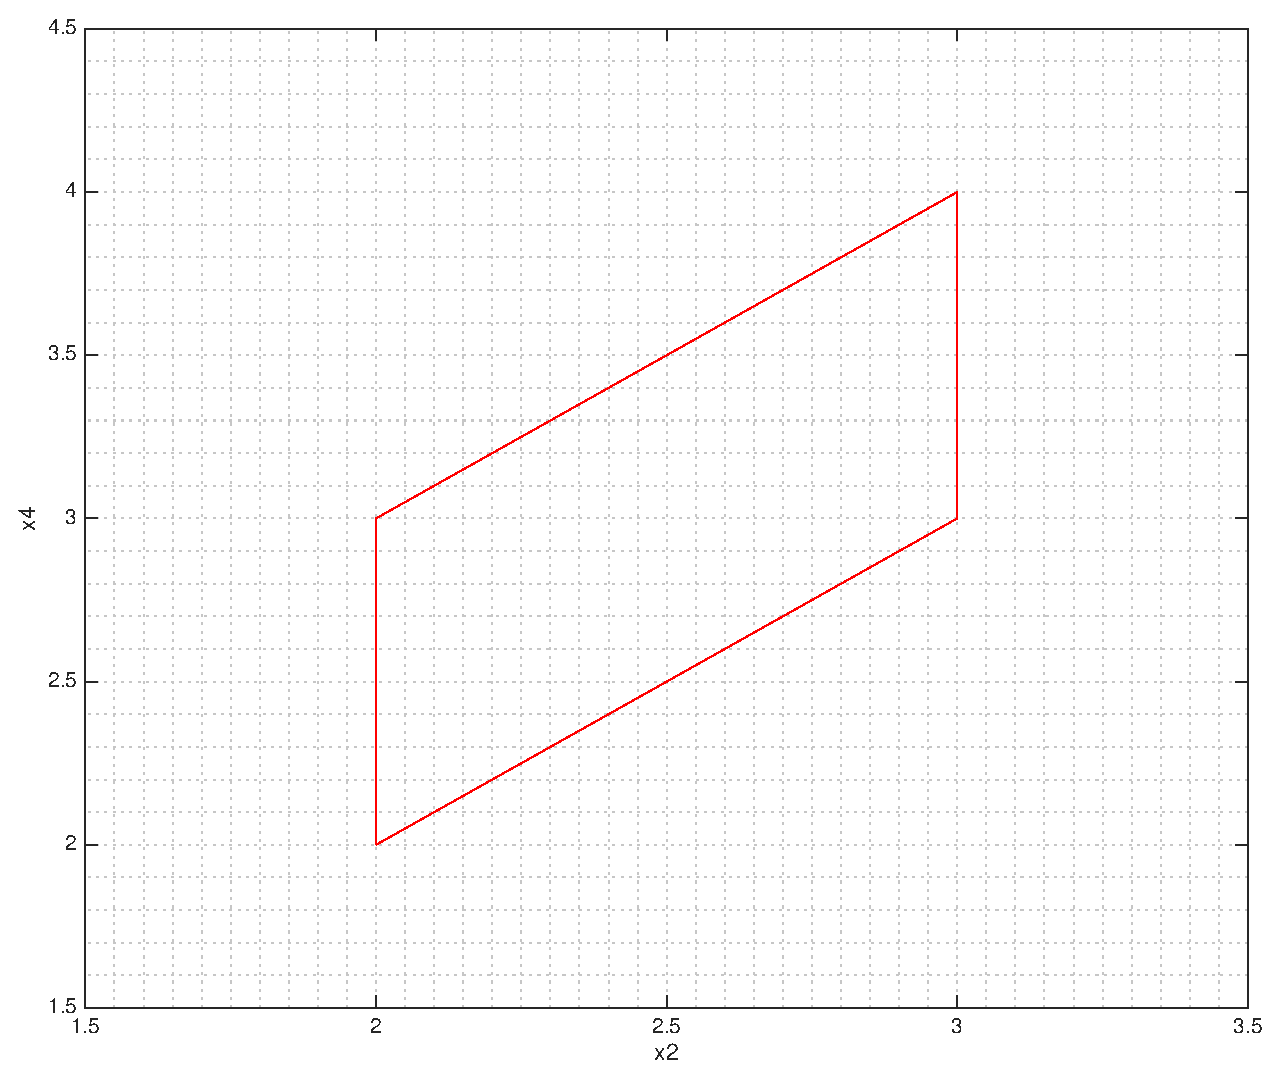
\includegraphics[width=0.55\textwidth]{P2P4.eps}}
\caption{Множество положений равновесия.}
\end{figure}
\FloatBarrier

Наша задача состоит в исследовании возможности перевода системы \RS во множество $\bar P$ при кусочно-непрерывном управлении из $U_1^*, U_2^*.$ 

% ---------- ПИ ----------

В работе \cite{MathBio} найден первый интеграл четырехмерной системы без управления: 
$$K(x) = x_1 - P_1\ln x_1 + \frac{b_1}{c_2}(x_2 - P_2\ln x_2) + \frac{b_1b_2}{c_2c_3}(x_3 - P_3\ln x_3) + \frac{b_1b_2b_3}{c_2c_3c_4}(x_4 - P_4\ln x_4).$$

Подставив вместо $P\, P(u),$ получим функцию, которая будет являться первым интегралом системы \RS при постоянном управлении:
\beq
	K(x|u) = x_1 - P_1\ln x_1 + \frac{b_1}{c_2}(x_2 - P_2(u)\ln x_2) + \frac{b_1b_2}{c_2c_3}(x_3 - P_3\ln x_3) + \frac{b_1b_2b_3}{c_2c_3c_4}(x_4 - P_4(u)\ln x_4).
\eeq

Будем рассматривать $K(x|u)$ как функцию фазовой переменной с параметром $u.$ Докажем, что она сильно выпукла и имеет минимум в точке $(P(u)).$

\begin{statement}
\label{compact}
	Функция $K(x|u)$ сильно выпукла на любом выпуклом ограниченном подмножестве $\mathbb{R}_+^4,$ а ее глобальный минимум достигается в точке $P(u).$
\end{statement}
\begin{Proof}
	Рассмотрим гессиан функции $K(x|u):$
	$$H = \text{diag} \left(\frac{P_1}{x_1^2}, \; \frac{P_2(u)b_1}{c_2x_2^2}, \; \frac{P_3b_1b_2}{c_2c_3x_3^2}, \; \frac{P_4(u)}{c_2c_3c_4x_4^2}\right).$$
	Очевидно, он больше нуля при всех $x_i > 0,$ следовательно, функция выпукла.\\
	Обозначим 
	$$K_1(x_1) = x_1 - P_1\ln x_1, \; K_2(x_2|u) = \frac{b_1}{c_2}(x_2 - P_2(u)\ln x_2),$$
	$$K_3(x_3) = \frac{b_1b_2}{c_2c_3}(x_3 - P_3\ln x_3), \; K_4(x_4|u) = \frac{b_1b_2b_3}{c_2c_3c_4}(x_4 - P_4(u)\ln x_4),$$ тогда $K(x|u) =  K_1(x_1) + K_2(x_2|u) + K_3(x_3) + K_4(x_4|u).$  Поскольку 
	$$K_1'(x_1) = 1 - \frac{P_1}{x_1}, \; K_2'(x_2|u) = \frac{b_1}{c_2} - \frac{P_2(u)b_1}{c_2x_2},$$
	$$K_3'(x_3) = \frac{b_1b_2}{c_2c_3} - \frac{b_1b_2P_3}{c_2c_3x_3}, \; K_4'(x_4|u) = \frac{b_1b_2b_3}{c_2c_3c_4} - \frac{b_1b_2b_3P_4(u)}{c_2c_3c_4x_4},$$ 
	глобальный минимум $K_i$ достигается при $x_i = P_i,$ следовательно, глобальный минимум $K(x|u)$ достигается в точке $P(u).$ \\
	 Докажем сильную выпуклость. Возьмем $x_i \leqslant \mu, i = \ftw{1}{4}, \text{где } \mu \geqslant \max\Set{P_i}{i = \ftw{1}{4}}.$ Тогда $H \geqslant \delta\cdot I,$ где  
	 $$\delta = \min\left(P_1, \frac{P_2(u)b_1}{c_2}, \frac{P_3b_1b_2}{c_2c_3}, \frac{P_4(u)b_1b_2b_3}{c_2c_3c_4}\right)/\mu^2.$$
	 Таким образом $\langle Hx,x \rangle \geqslant \langle \delta Ix,x \rangle = \delta \|x\|^2,$ что и завершает доказательство.
\end{Proof}

{\bf Следствие.} Приближение к положению равновесия равносильно уменьшению $K(x|u).$\\

%Особые режимы

	Если рассматривать задачу быстродействия для данной системы, то ниже доказано утверждение, которое говорит о том, что особых режимов принципа максимума Понтрягина нет.

\begin{statement}
	В системе (1) в области $\mathbb{R}_+^4$ не могут возникать особые режимы управления.
\end{statement}
\begin{Proof}
    Выпишем функцию Гамильтона-Понтрягина для нашей системы.
        $$H(\psi, x, u) = \psi_1x_1(r_1 + u_1 - b_1x_2) + \psi_2x_2(-r_2 - b_2x_3 + c_2x_1) + \psi_3x_3(-r_3 + u_2 - b_3x_4 + c_3x_2) + \psi_4x_4(-r_4 + c_4x_3),$$
    
    где  $\psi(t) \in C, \; \psi(t) \ne 0 \; \text{и удовлетворяет сопряженной системе системе:}$
    
    $$
    \left\{
    \begin{aligned}
    	\dot \psi_1 &= -(\psi_1(r_1 + u - b_2x_2) + \psi_2x_2c_2), \\
    	\dot \psi_2 &= -(-b_1\psi_1x_1 + \psi_2(-r_2 - b_2x_3 + c_2x_1) + \psi_3x_3c_3), \\
    	\dot \psi_3 &= -(-b_2\psi_2x_2 + \psi_3(-r_3 + u_2 - b_3x_4 + c_3x_2) + \psi_4x_4c_4), \\
    	\dot \psi_4 &= -(b_3\psi_3x_3 + \psi_4(-r_4 + c_4x_3)).
    \end{aligned}
    \right.
    $$
    
    Из принципа максимума для задачи быстродействия $H(\psi(t), x(t), u^*(t)) = \sup\limits_{u \in U^*} H(\psi,x,u).$
    
    Посчитаем производную $H$ по $u:$
    
    $$H'_u = (\psi_1x_1, \psi_3x_3) \text{ откуда } u_1^* = \begin{cases} u_1^{max}, & \psi_1x_1 \geqslant 0, \\  u_1^{min}, & \psi_1x_1 < 0.\end{cases}, \;\; u_2^* = \begin{cases} u_2^{max}, & \psi_3x_3 \geqslant 0, \\  u_2^{min}, & \psi_3x_3 < 0.\end{cases}$$
    
    Особый режим будет возникать, если хотя бы одна из компонент управления определяется неоднозначно, то есть либо $\psi_1x_1 = 0,$ либо $\psi_3x_3 = 0$ на ненулевом промежутке времени.
    Так как в нашей системе $x_1$ и $x_3$ положительны, учитываются только $\psi_1, \psi_3.$  
    
    Рассмотрим оба варианта.
    \begin{enumerate}
    \item
        	Пусть $\psi_1(t) = 0, t \in [t_1 t_2].$ Рассмотрим последовательно $\dot \psi_i$ и убедимся, что все сопряженные переменные нулевые.
        
        Если $\psi_1(t) = 0$ на промежутке $[t_1, t_2],$ то $\dot \psi_1 = 0$ на этом же временном отрезке. Но тогда из первого сопряженного уравнения $\psi_2 = 0,$ следовательно и $\dot \psi_2 = 0, \;  t \in [t_1, t_2],$ а тогда из второго сопряженного уравнения $\psi_3 = 0, \;  t \in [t_1, t_2].$ Аналогично $\dot \psi_3 = 0, \;  t \in [t_1, t_2]$ и из третьего сопряженного уравнения $\psi_4 = 0, \;  t \in [t_1, t_2],$ что противоречит невырожденности $\psi(t).$
        
    \item
    	Пусть $\psi_3(t) = 0, \psi_1(t) \ne 0, t \in [t_1 t_2],$ тогда и $\dot \psi_3(t) = 0$ на том же временном отрезке. Таким образом $-b_2\psi_2x_2 + \psi_4x_4c_4 = 0.$ Возьмем производную по времени от этого выражения:
    	\begin{multline*}
    		0 = -b_2(\dot \psi_2x_2 + \psi_2 \dot x_2) + c_4(\dot \psi_4 x_4 + \psi_4 \dot x_4) = \\
    		= -b_2(-x_2(-b_1\psi_1x_1 + \psi_2(-r_2 - b_2x_3 + c_2x_1)) + \psi_2 x_2(-r_2 - b_2x_3 + c_2x_1)) + \\
    		+ c_4(\psi_4x_4(-r_4 + c_4x_3) + \psi_4x_4(-r_4 + c_4x_3)) = -b_1b_2x_1x_2\psi_1.
    	\end{multline*}
    	
    	Но $x_1, x_2, \psi_1 \ne 0,$ а значит, мы получили противоречие, что и завершает доказательство.
    
    \end{enumerate}    
\end{Proof}

	Решая поставленную задачу, пользоваться ПМП затруднительно в силу фактической невозможности проинтегрировать соответствующую гамильтонову систему или хотя бы получить какую-то информацию о поведении ее траекторий. Поэтому далее мы будем пользоваться другой схемой решения. Как будет показано ниже, в системе возникают скользящие режимы, что говорит о том, что соответствующие траектории не будут являться оптимальными по быстродействию, однако будет доказано, что мы можем решить задачу за конечное время.

\section{Синтез управления с применением первого интеграла системы}

	Предложен способ построения управления таким образом, чтобы уменьшать $K(x|u)$ и тем самым приближаться к положению равновесия. Метод несколько схож с методом функций Ляпунова, изложенным в классической работе \cite{Lyapunov}. 
%Вернемся к нашим баранам
Посчитаем производную $\frac{dK(x|u^0)}{dt}$ при некотором $u^0 = (u_1^0, u_2^0)$ в силу системы \RS:

\begin{multline*}
    \frac{dK(x|u_0)}{dt} = \dd{K(x|u_0)}{x_1}\dot x_1 + \dd{K(x|u_0)}{x_2}\dot x_2 + \dd{K(x|u_0)}{x_3}\dot x_3 + \dd{K(x|u_0)}{x_4}\dot x_4 = \\
    = -\frac{1}{c_2c_3c_4}\left((u_2 - u_2^0)(b_1b_2(r_4 - c_4x_3)) + c_3(u_1 - u_1^0)(b_2r_4 + c_4r_2 - c_2c_4x_1)\right) = \\
    = \frac{b_1b_2}{c_2c_3}(u_2 - u_2^0)(x_3 - P_3) + (u_1 - u_1^0)(x_1 - P_1) \to \min\limits_{u_1 \in U_1^*, u_2 \in U_2^*}
\end{multline*}

Заметим, что равновесие по $x_1$ и $x_3$ разделяет все пространство на четыре области, в каждой из которых будет свой минимизатор.
\begin{enumerate}
\item
	В области $x_1 > P_1, \, x_3 > P_3$ производная будет минимальной при $u_1 = u_1^{min}, \, u_1^0 = u_1^{max}, \, u_2 = u_2^{min}, \, u_2^0 = u_2^{max}.$
\item
	В области $x_1 > P_1, \, x_3 < P_3$ производная будет минимальной при $u_1 = u_1^{min}, \, u_1^0 = u_1^{max}, \, u_2 = u_2^{max}, \, u_2^0 = u_2^{min}.$
\item
	В области $x_1 < P_1, \, x_3 > P_3$ производная будет минимальной при $u_1 = u_1^{max}, \, u_1^0 = u_1^{min}, \, u_2 = u_2^{min}, \, u_2^0 = u_2^{max}.$
\item
	В области $x_1 < P_1, \, x_3 < P_3$ производная будет минимальной при $u_1 = u_1^{max}, \, u_1^0 = u_1^{min}, \, u_2 = u_2^{max}, \, u_2^0 = u_2^{min}.$
\end{enumerate}

Введем 4 функции:
$$K_1(x) = K(x|u_1^{min}, u_2^{min}), \, K_2(x) = K(x|u_1^{max}, u_2^{min}),$$ 
$$K_3(x) = K(x|u_1^{min}, u_2^{max}), \, K_4(x) = K(x|u_1^{max}, u_2^{max}).$$

Беря управление, минимизирующее производную $\frac{dK(x|u^0)}{dt}$ в соответствующей области, мы будем уменьшать три функции, а четвертая будет постоянной. Процесс будет повторяться до тех пор, пока мы не попадем на положение равновесия, где все четыре функции станут постоянными. 

\begin{figure}[h]
\center{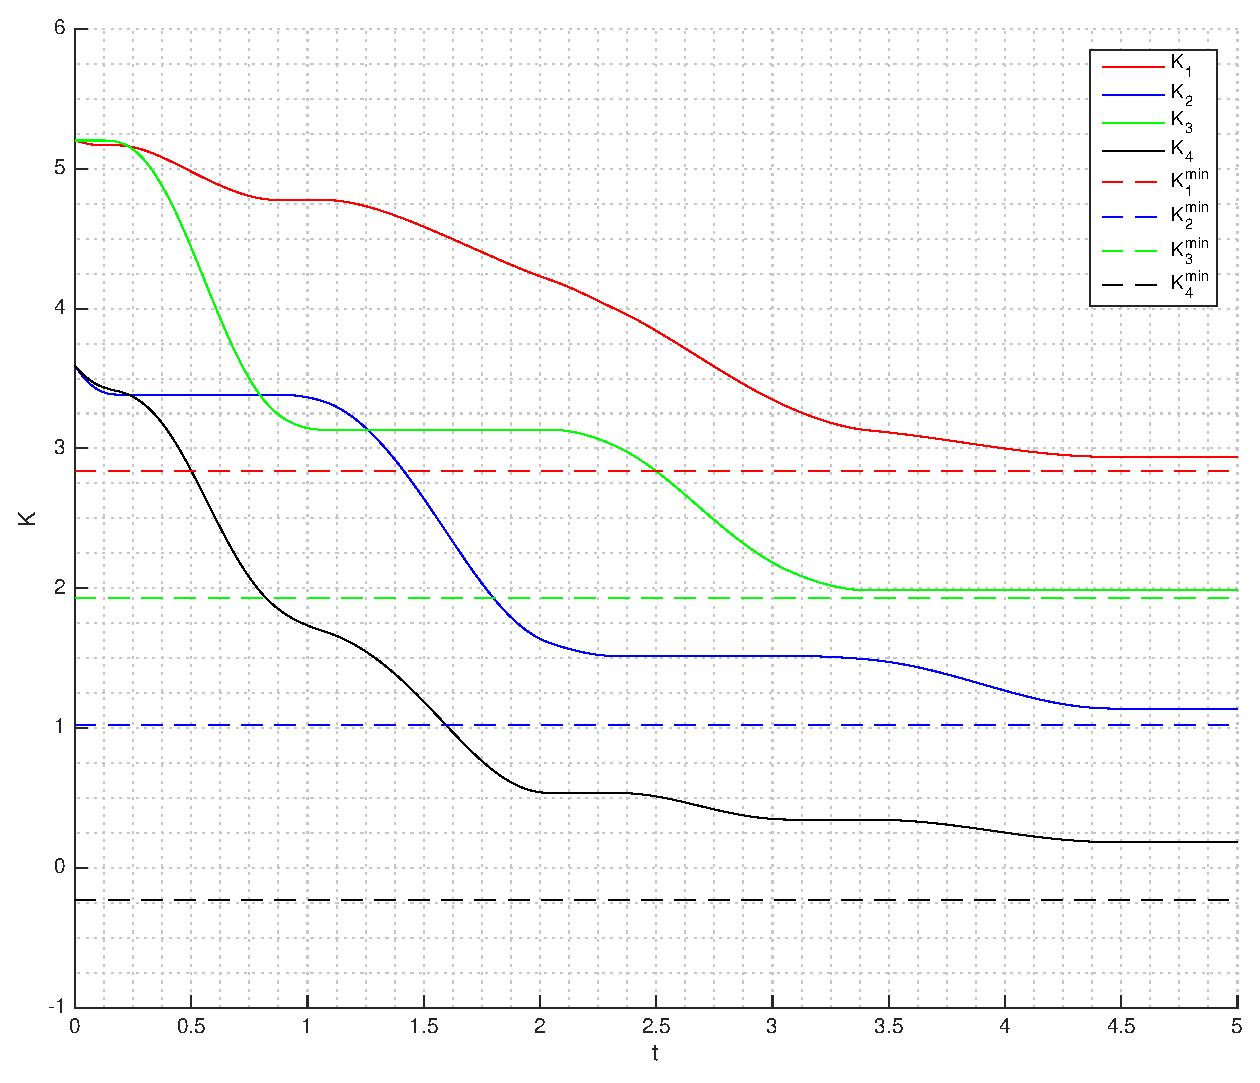
\includegraphics[width=0.5\textwidth]{Kord1.eps}}
\caption{$K_i(x|u), i = \overline{1,4}$.}
\end{figure}
\FloatBarrier

Соответствующие фазовые координаты:

\begin{figure}[h]
\center{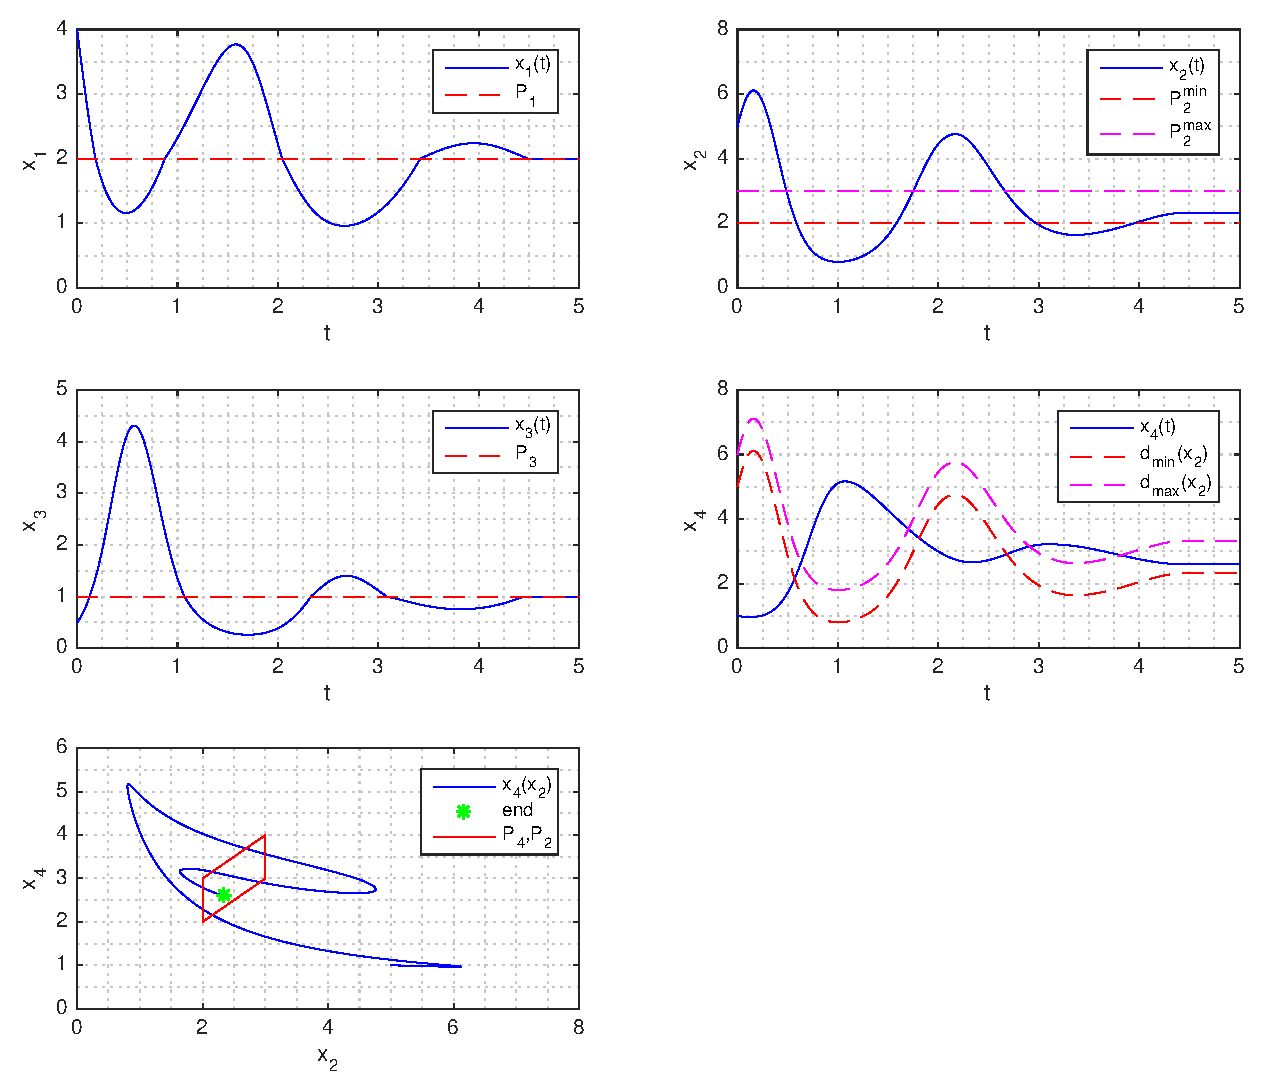
\includegraphics[width=0.6\textwidth]{ord1.eps}}
\caption{Фазовые координаты.}
\end{figure}
\FloatBarrier

\begin{figure}[h]
\center{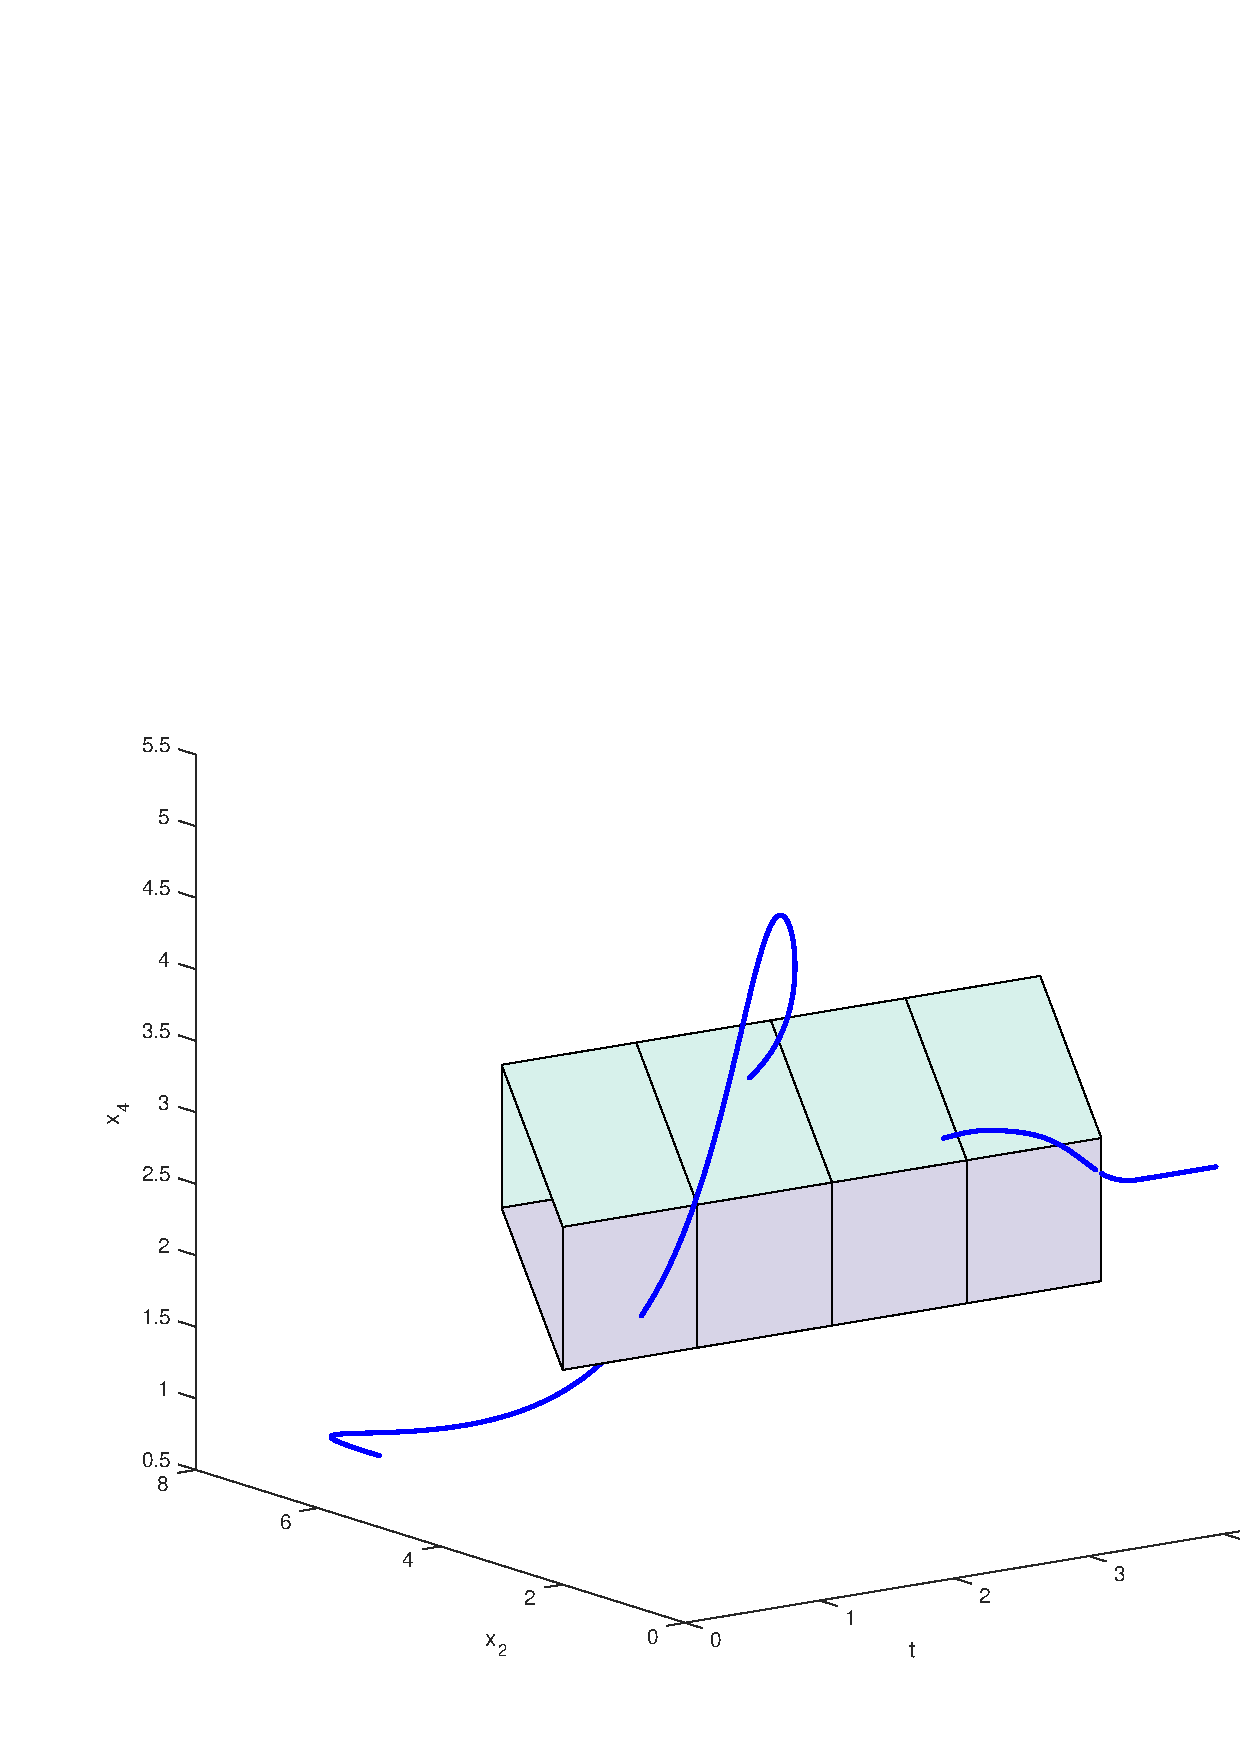
\includegraphics[width=0.6\textwidth]{3D.png}}
\caption{Траектория в терминах $(t,x_2,x_4)$.}
\end{figure}
\FloatBarrier


%=========Скользящие режимы========
\section{Скользящие режимы} 
	\indent Особенностью этого метода является то, что неопределенность возникает на самих гиперповерхностях $x_1 = P_1, x_3 = P_3.$ В \cite{Filippov} рассмотрены дифференциальные уравнения с разрывной правой частью, в которых возникают скользящие режимы. Рассмотрим, в каких случаях они возникают в нашей системе, и регуляризуем скользящий режим таким образом, чтобы не уходить с линии переключения.

	Для начала кратко опишем, в каких случаях в системе дифференциальных уравнений возникают скользящие режимы, и приведем описание метода Филиппова.

	Перепишем систему в виде:
$$\dot x(t) = \begin{cases} f_1(x), & \sigma(x,t) < 0 \\ f_2(x), & \sigma(x,t) > 0,\end{cases}$$
	где $\sigma(x,t) = 0$ --- поверхность разрыва правой части уравнения.

	Необходимое и достаточное условие скользящего режима на отрезке $x \in [a, b]$ в этом случае будет:

$$
\left\{
\begin{aligned}
    \lim_{\sigma \to 0+0}\dd{\sigma(x,t)}{x} f_2(x) < 0 \\
    \lim_{\sigma \to 0-0} \dd{\sigma(x,t)}{x} f_1(x) > 0.
\end{aligned}
\right.
\;\;\; \forall x \in [a, b] \subset \Set{x}{\sigma(x,t) = 0}
$$

	Таким образом мы можем рассматривать динамическую систему следующего вида:
$$\dot x(t) = \begin{cases} f_1(x), & \sigma(x,t) < 0 \\ f_s(x), & \sigma(x,t) = 0 \\ f_2(x), & \sigma(x,t) > 0.\end{cases}$$

 	Для этого применим метод продолжения Филиппова:

$$f_s(x) = \alpha f_1(x) + (1 - \alpha) f_2(x), \text{  где}$$
$$\alpha \in [0, 1] : \dd{\sigma(x,t)}{x} f_s(x) = 0$$
$$\alpha = \frac{\langle \nabla(\sigma), f_1\rangle}{\langle \nabla(\sigma), f_1 - f_2 \rangle}.$$

	В этом случае мы будем выбирать управление $u = u^c$ таким образом, чтобы двигаться вдоль поверхности $\sigma(x,t) = 0$ некоторое положительное время, а именно, до того момента, когда нарушится условие скользящего режима.

	Будем рассматривать отдельно случай скользящего режима по первой координате и по третьей.

% ------ Скользящий режим по х_1 -------
\subsection{Скользящий режим по $x_1$.}
\begin{statement}
	Пусть в \RS нет скользящего режима по $x_3$. Тогда скользящий режим по $x_1$ возникает при 
	$$
        	\left\{
        \begin{aligned}
        		&x_1 = P_1, \\
        		&P_2(u_1^{min}) < x_2 < P_2(u_1^{max}).
        \end{aligned}
        \right.
	$$
	Если положить $u_1 = u_1^c = b_1x_2 - r_1,$ то разрыв в правой части будет устранен.
\end{statement}
\begin{Proof}\\
    \indent В этом случае 
    $f_1(x) = f(x, u_1^{max}, u_2^0), \; f_2(x) = f(x, u_1^{min}, u_2^0), \; \sigma(x,t) = x_1 - P_1.$
    Тогда $\dd{\sigma}{x} = [1,0,0,0]^T, \; \langle \dd{\sigma(x)}{x}, f_1(x) \rangle = x_1(r_1 + u_1^{max}  - b_1x_2), \; \langle \dd{\sigma(x)}{x}, f_2(x) \rangle = x_1(r_1 + u_1^{min}  - b_1x_2).$
    
    %$$
    %\left\{
    %\begin{aligned}
    %\label{system}
    %	f_1^1 &= x_1(r_1 + u_1^{max}- b_1x_2), \\
    %	f_1^2 &= x_2(-r_2 - b_2x_3 + c_2x_1), \\
    %	f_1^3 &= x_3(-r_3 + u_2^0 - b_3x_4 + c_3x_2), \\
    %	f_1^4 &= x_4(-r_4 + c_4x_3).
    %\end{aligned}
    %\right. \;\;
    %\left\{
    %\begin{aligned}
    %\label{system}
    %	f_2^1 &= x_1(r_1 + u_1^{min}- b_1x_2), \\
    %	f_2^2 &= x_2(-r_2 - b_2x_3 + c_2x_1), \\
    %	f_2^3 &= x_3(-r_3 + u_2^0 - b_3x_4 + c_3x_2), \\
    %	f_2^4 &= x_4(-r_4 + c_4x_3).
    %\end{aligned}
    %\right. \;\;\;\;
    %\sigma(x,t) = \sigma(x) = x_1 - P_1.
    %$$
    Мы предполагаем, что по $x_3$ скользящего режима нет, и вторая компонента управления определяется однозначно. Ниже будет доказано, что скольжение одновременно по обеим координатам эквивалентно решению исходной задачи.
    
    Получим, что скользящий режим возникает при 
    $$
    \left\{
    \begin{aligned}
    	\lim_{x_1 - P_1 \to 0 + 0} x_1(r_1 + u_1^{min} - b_1x_2) < 0, \\
    	\lim_{x_1 - P_1 \to 0 - 0} x_1(r_1 + u_1^{max} - b_1x_2) > 0, \\
    \end{aligned}
    \right.
    $$
    откуда $P_2(u_1^{min}) < x_2 < P_2(u_1^{max}).$
    
    То есть при таких $x_2$, если мы находимся вблизи гиперповерхности $x_1 = P_1$ с соответствующей стороны, у нас возникает по первой координате скользящий режим. Тогда, применяя метод Филиппова, получим 
    $$
    \dot x(t) = \begin{cases} f_1(x), & \sigma(x,t) < 0 \\ \alpha_1 f_1(x) + (1 - \alpha_1) f_2(x), & \sigma(x,t) = 0 \\ f_2(x), & \sigma(x,t) > 0\end{cases} \; \Leftrightarrow \; \dot x(t) = \begin{cases} f(x,u_1^{max}, u_2^0), & \sigma(x,t) < 0 \\ f(x, u_1^c, u_2^0), & \sigma(x,t) = 0 \\ f(x, u_1^{min}, u_2^0), & \sigma(x,t) > 0,\end{cases}
    $$
    
    где
    
    $$\alpha_1 = \frac{r_1 + u_1^{max} - b_1x_2}{u_1^{max} - u_1^{min}},$$
    $$u_1^c = \alpha_1 u_1^{min} + (1-\alpha_1)u_1^{max} = b_1x_2 - r_1.$$

\end{Proof}

% ------ Скользящий режим по х_3 -------
\subsection{Скользящий режим по $x_3$.}
	
	Приведем аналогичное утверждение про скользящий режим по третьей координате.
\begin{statement}
	Пусть в \RS нет скользящего режима по $x_1$. Тогда скользящий режим по третьей координате возникает, если 
	$$
	\left\{
	\begin{aligned}
		&x_3 = P_3, \\
		&d_{min}(x_2) = \frac{c_3x_2 - r_3 + u_2^{min}}{b_3} < x_4 < \frac{c_3x_2 - r_3 + u_2^{max}}{b_3} = d_{max}(x_2).
	\end{aligned}
	\right.
	$$
	Если положить $u_2 = u_2^c = r_3 + b_3x_4 - c_3x_2,$ то разрыв в правой части будет устранен. 
\end{statement}
\begin{Proof}
    	\indent В этом случае $f_1(x) = f(x, u_1^0, u_2^{max}), \; f_2(x) = f(x, u_1^0, u_2^{min}), \; \sigma(x,t) = x_3 - P_3.$
    Тогда $\dd{\sigma}{x} = [0,0,1,0]^T, \; \langle \dd{\sigma(x)}{x}, f_1(x) \rangle = x_3(-r_3 + u_2^{max}  - b_3x_4 + c_3x_2), \; \langle \dd{\sigma(x)}{x}, f_2(x) \rangle = x_3(-r_3 + u_2^{min}  - b_3x_4 + c_3x_2).$
    Получим, что скользящий режим возникает при 
    $$
    \left\{
    \begin{aligned}
    	\lim_{x_3 - P_3 \to 0 + 0} x_3(-r_3 + u_2^{min}  - b_3x_4 + c_3x_2) < 0, \\
    	\lim_{x_3 - P_3 \to 0 - 0} x_3(-r_3 + u_2^{max}  - b_3x_4 + c_3x_2) > 0, \\
    \end{aligned}
    \right.
    $$
    откуда $d_{min}(x_2) = \frac{c_3x_2 - r_3 + u_2^{min}}{b_3} < x_4 < \frac{c_3x_2 - r_3 + u_2^{max}}{b_3} = d_{max}(x_2).$
    
    	После регуляризации получаем
    $$
    \dot x(t) = \begin{cases} f(x,u_1^0, u_2^{max}), & \sigma(x,t) < 0 \\ f(x, u_1^0, u_2^c), & \sigma(x,t) = 0 \\ f(x, u_1^0, u_2^{min}), & \sigma(x,t) > 0,\end{cases}
    $$
    
    где
    
    $$\alpha_2 = \frac{-r_3 + u_2^{max} - b_3x_4 + c_3x_2}{u_2^{max} - u_2^{min}},$$
    $$u_2^c = \alpha_2 u_2^{min} + (1-\alpha_2)u_2^{max} = r_3 + b_3x_4 - c_3x_2.$$
\end{Proof}

\begin{Remark_s} Мы рассматриваем скользящие режимы либо по первой, либо по третьей координате, так как в случае одновременного скольжения по обеим координатам задача решена. 
\end{Remark_s}
\begin{Proof}
	\indent Пусть имеет место скользящий режим по обеим координатам. То есть
	$$
		\left\{
		\begin{aligned}
			x_1 &= P_1, \\
			x_2 &\in [P_2^{min}, P_2^{max}], \\
			x_3 &= P_3, \\
			x_4 &\in [d_{min}(x_2), d_{max}(x_2)].
		\end{aligned}
		\right.
	$$
	Так как по первой и по третьей координате мы двигаемся вдоль $x_1 = P_1\text{ и } x_3 = P_3$ соответственно, то $\dot x_1 = 0 = \dot x_3.$ А так как $x_1 = P_1, x_3 = P_3,$ из системы \RS получим, что $\dot x_2 = 0 = \dot x_4,$ что и означает попадание в положение равновесие и полную стабилизацию системы.
\end{Proof}

\begin{Remark_s}
	Случай <<отталкивания>> от поверхностей разрыва правой части уравнения невозможен.
\end{Remark_s}

\begin{Proof} 
	\indent Необходимым условием для разнонаправленности векторного поля $f(x,u)$ вблизи поверхности разрыва будет 
    $$
    	\left\{
	\begin{aligned}
		x_2 &\geqslant P_2^{max}, \\
		x_2 &\leqslant P_2^{min}
	\end{aligned}
	\right.
    $$
    в первом случае и 
    $$
    	\left\{
	\begin{aligned}
		x_4 &\geqslant d^{max}(x_2), \\
		x_4 &\leqslant d^{min}(x_2)
	\end{aligned}
	\right.
    $$
    во втором. Очевидно, в обоих случаях требуемое невозможно, а значит, вблизи поверхностей $x_1 = P_1, x_3 = P_3$ возможно либо непрерывное векторное поле $f(x,u),$ либо случаи скользящих режимов по одной из координат, рассмотренные выше.

\end{Proof}
%sliding behaviour

%=========Конечность процесса=========

\section{Конечность процесса}

	 Докажем, что за конечное время мы придем в $\varepsilon$-окрестность равновесия.
	
\begin{Def} Назовем $\alpha\varepsilon$-окрестностью положения равновесия множество 
	$$\bar P_{\bar\alpha}^{\varepsilon} = \left\{x \in \mathbb{R}^4 \;:\;|x_1 - P_1| \leqslant \alpha_1\varepsilon, |x_3 - P_3| \leqslant  \alpha_3\varepsilon, x_2 \in [P^{min}_2 -  \alpha_2\varepsilon, P^{max}_2 +  \alpha_2\varepsilon],\right.$$
	$$\left. x_4 \in [d^{min}(x_2) -  \alpha_4\varepsilon, d^{max}(x_2) +  \alpha_4\varepsilon]\right\}.$$
\end{Def}

Будем обозначать попадание в соответствующую $\alpha_i\varepsilon$-окрестность по $i$-ой координате $P_{\alpha_i i}^{\varepsilon}.$

% -------- Лемма1 --------

\begin{lemma} 
\label{dkdt}
	$$\forall \delta_1 > 0, \delta_3 > 0 \;\exists A = A(\delta_1, \delta_2) \;:\; $$ $$\left|\frac{dK(x|u)}{dt}\right| > A \;\; \forall x \in \Set{\bar x}{x_2, x_4 \in \mathbb{R}, |x_1 - P_1| > \delta_1 \text{или } |x_3 - P_3| > \delta_3}$$
\end{lemma}
\begin{Proof}
	Если $|x_1 - P_1| > \delta_1$ или $|x_3 - P_3| > \delta_3,$ то 

    $$
    	\min\limits_u\frac{dK(x|u)}{dt} \leqslant \begin{cases} -a_1 = -\delta_1(u_1^{max} - u_1^{min}), &  |x_1 - P_1| > \delta_1 \\ -a_2 = -\delta_3\frac{b_1b_2}{c_2c_3}(u_2^{max} - u_2^{min}), & |x_3 - P_3| > \delta_3, \end{cases}
    $$
    т.е.
    $$\min\limits_u\frac{dK(x|u)}{dt} \leqslant \min(-a_1, -a_2) =  A.$$
    Таким образом мы в явном виде нашли A, чем и завершили доказательство.
\end{Proof}

% ----------Лемма 2 -------------

\begin{lemma}
\label{delta_t}
	Пусть $x_2(t_0) \not \in P_{\alpha_2 \,2}^{\varepsilon}, \; 0 \leqslant \alpha'_2 < \alpha_2,$ 
	тогда $\exists \Delta t > 0 \;:\; \forall t \in [t_0, t_0 + \Delta t) \; x_2(t) \not \in P_{\alpha'_2 \,2}^{\varepsilon}.$ 
\end{lemma}
\begin{Proof}
%	Введем $$v_2^{min} = \min\Set{-r_2 - b_2x_3 + c_2x_1}{K(x|u) \leqslant K(x^0,u)},$$
%	$$v_2^{max} = \max\Set{-r_2 - b_2x_3 + c_2x_1}{K(x|u) \leqslant K(x^0,u)}.$$ Тогда $x_2 v_2^{min} \leqslant \dot x_2 \leqslant x_2 v_2^{max}.$Оценим время, которое понадобится $x_2,$ чтобы дойти до до $P_2$.
%	Пусть $x_2 > P_2^{max} + \alpha_2\varepsilon.$ Тогда $\frac{d}{dt}\ln x_2 \geqslant v_2^{min}.$ Проинтегрировав до момента, когда $x_2 = P_2^{max}$, получим, что $\ln P_2^{max} - \ln (P_2^{max} + \alpha_2\varepsilon) \geqslant v_2^{min}\Delta t_1,$ откуда, с учетом, что $v_2^{min} < 0,$ искомая оценка времени будет $$\Delta t_1 \geqslant \frac{\ln \frac{P_2^{max}}{P_2^{max} + \alpha_2\varepsilon}}{v_2^{min}}.$$
%	Аналогично оценим время в случае, когда $x_2 < P_2^{min} - \alpha_2\varepsilon:$
%	$$\Delta t_2 \geqslant \frac{\ln \frac{P_2^{min}}{P_2^{min} + \alpha_2\varepsilon}}{v_2^{max}}.$$
	Введем $$v_2^{min} = \min\Set{x_2(-r_2 - b_2x_3 + c_2x_1)}{K(x|u) \leqslant K(x^0,u)},$$
	$$v_2^{max} = \max\Set{x_2(-r_2 - b_2x_3 + c_2x_1)}{K(x|u) \leqslant K(x^0,u)}.$$ 
	По Утверждению \ref{compact} $K(x|u)$ --- выпукла, из \cite{Vasiliev} ее множество уровня --- компакт, следовательно, на нем будут достигаться минимум и максимум непрерывной функции. Тогда $v_2^{min} \leqslant \dot x_2 \leqslant v_2^{max}.$ Оценим время, которое понадобится $x_2,$ чтобы дойти до $P_{\alpha'_2\,2}^{\varepsilon}$.
	Пусть $x_2 > P_2^{max} + \alpha_2\varepsilon.$ Тогда $\frac{d}{dt}x_2 \geqslant v_2^{min}.$ Проинтегрировав до момента, когда $x_2 = P_2^{max} + \alpha'_2\varepsilon$, получим, что $P_2^{max} + \alpha'_2\varepsilon - (P_2^{max} + \alpha_2\varepsilon) \geqslant v_2^{min}\Delta t^1_2,$ откуда, с учетом, что $v_2^{min} < 0,$ искомая оценка времени будет $$\Delta t^1_2 \geqslant \frac{(\alpha'_2 - \alpha_2)\varepsilon}{v_2^{min}}.$$
	Аналогично оценим время в случае, когда $x_2 < P_2^{min} - \alpha_2\varepsilon:$
	$$\Delta t^2_2 \geqslant \frac{(\alpha_2 - \alpha'_2)\varepsilon}{v_2^{max}}.$$

	Таким образом, мы оценили $\Delta t_2 = \min(\Delta t^1_2, \Delta t^2_2) = (\alpha_2 - \alpha'_2)\varepsilon\min(\frac{1}{v_2^{max}}, -\frac{1}{v_2^{min}})$ --- минимальное время, за которое $x_2$ дойдет до $\alpha'_2\varepsilon$-окрестности $P_2,$ если она находилась вне $\alpha_2\varepsilon$-окрестности $P_2.$
\end{Proof}

\begin{Remark_l}
\label{rem_1}
	 Аналогично можно оценить минимальное время $\Delta t_1, \Delta t_3,$ за которое $x_1$ и $x_3$ дойдут из $P_{\alpha'_1 \, 1}^{\varepsilon} \text{ и } P_{\alpha'_3 \, 3}^{\varepsilon}$ до $P_{\alpha_1 \, 1}^{\varepsilon} \text{ и } P_{\alpha_3 \, 3}^{\varepsilon}$ соответственно, где $0 <\alpha'_i < \alpha_i, \; i = 1,3.$
\end{Remark_l}

Положим в дальнейшем $\alpha_1 = 1 = \alpha_3.$

% ---------------- Лемма 3 ------------

\begin{lemma}
\label{alpha_2}
	Пусть $|x_1(t_0) - P_1| < \varepsilon.$
	Тогда $\exists \alpha_2 \;:$ если $x_2(t_0) \not \in P_{\alpha_2 \, 2}^{\varepsilon},$ то
$\exists t > t_0 : x_1(t) \not \in [P_1 - \varepsilon, P_1 + \varepsilon].$
\end{lemma}
\begin{Proof}
	Оценим скорость $x_1.$ Для этого разделим промежуток времени, когда $x_2$ находится вне $P_2$ на две части: 
	\begin{enumerate}
		\item $x_2 > P_2^{max} + \frac{\alpha_2\varepsilon}{2}$ или $x_2 < P_2^{min} - \frac{\alpha_2\varepsilon}{2}$,
		\item $x_2 \in [P_2^{min} - \frac{\alpha_2\varepsilon}{2}, P_2^{max} + \frac{\alpha_2\varepsilon}{2}].$
	\end{enumerate}
	Будем рассматривать первый промежуток. Для него по Лемме \ref{delta_t}, положив $\alpha'_2 = \frac{\alpha_2}{2},$ найдем $\Delta t_2$ --- минимальное время, которое $x_2$ будет находиться в границах из пункта 1. Тогда, считая $\varepsilon$ настолько маленьким, чтобы $P_1 - \varepsilon > 0,$
	$$|\dot x_1| = |x_1(r_1 +u_1 - b_1x_2)| = |x_1b_1(P_2(u) - x_2)| > \frac{\alpha_2}{2}b_1\varepsilon(P_1 - \varepsilon).$$ 
	Оценим расстояние, которое пройдет за это время $x_1:$
	$$S_{x_1} > \frac{\alpha_2}{2}b_1\varepsilon(P_1 - \varepsilon) \Delta t_2.$$
	Потребуем, чтобы оно было больше $2\varepsilon$ и выведем оценку на $\alpha_2:$
	$$S_{x_1} \geqslant 2 \varepsilon \; \Rightarrow \; \alpha_2 \geqslant \frac{4\varepsilon}{(P_1 - \varepsilon)\varepsilon b_1\Delta t_2},$$
	где $\Delta t_2 = \frac{\alpha_2}{2}\varepsilon\min(\frac{1}{v_2^{max}}, -\frac{1}{v_2^{min}}),$ откуда 
	$$(\alpha_2)^2 \geqslant \frac{8}{(P_1 - \varepsilon)\varepsilon b_1v_2^0},$$
	где $v_2^0 = \min(\frac{1}{v_2^{max}}, -\frac{1}{v_2^{min}}).$\\
	Таким образом мы в явном виде получили оценку на искомое $\alpha_2,$ что и завершает доказательство.
\end{Proof}

\begin{Remark_l} 
\label{rem_2}
Аналогичные Леммам \ref{delta_t}, \ref{alpha_2} утверждения можно доказать и в случае 
$$|x_3 - P_3| < \alpha_3\varepsilon, \; x_4 \in [d_{min}(x_2) - \alpha_2\varepsilon, d_{max}(x_2) + \alpha_2\varepsilon].$$ Поэтому приведем лишь моменты, которые будут отличаться для $x_2$ и $x_4.$
Отличие будет в оценке скорости для $x_4$, где $v_4^{min}, v_4^{max}$ следует определить следующим образом: 
$$v_4^{min} = \min\Set{x_4(-r_4 + c_4x_3)}{K(x|u) \leqslant K(x^0,u)} - \frac{c_3}{b_3}v_2^{max},$$
$$v_4^{max} = \max\Set{x_4(-r_4 + c_4x_3)}{K(x|u) \leqslant K(x^0,u)} - \frac{c_3}{b_3}v_2^{min},$$
так как мы оцениваем скорость сближения $x_4$ и $d_2.$ \\
Тогда $\Delta t_4 \geqslant \min(\Delta t^1_4, \Delta t^2_4) = \frac{\alpha_4}{2}\varepsilon v_4^0,$ где 
$v_4^0 = \min(\frac{1}{v_4^{max}}, -\frac{1}{v_4^{min}}).$ В таком случае $\alpha^2_4 \geqslant \frac{8}{(P_3 - \varepsilon)\varepsilon b_3v_4^0}.$
\end{Remark_l}

\begin{figure}[h]
\center{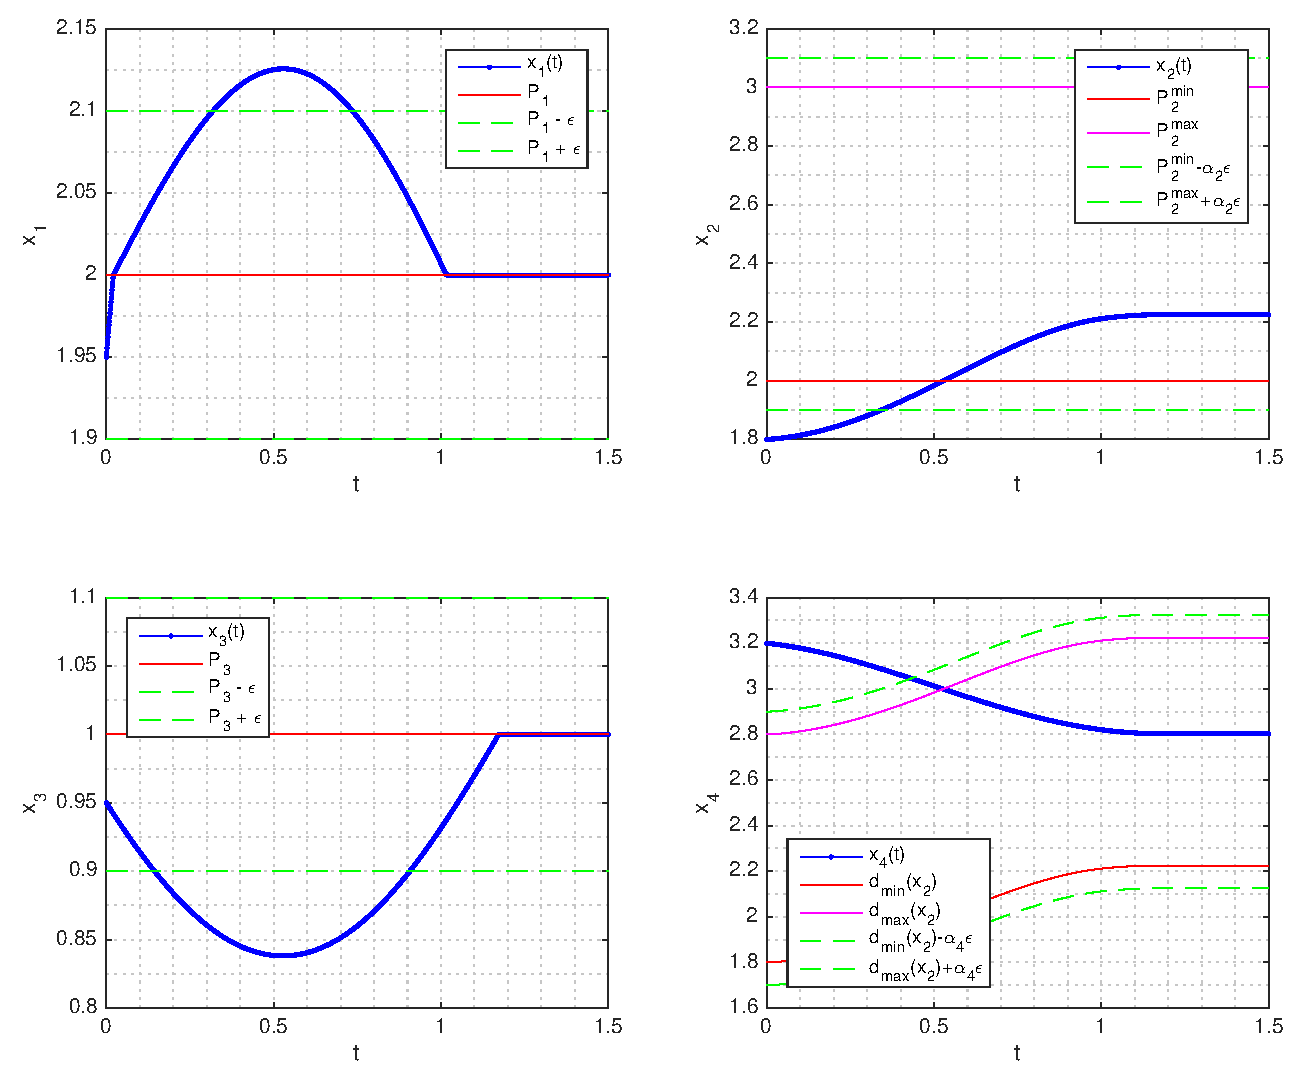
\includegraphics[width=0.7\textwidth]{eps1.eps}}
\caption{Случай из Леммы \ref{alpha_2}.}
\end{figure}
\FloatBarrier

Теперь мы готовы сформулировать основной результат работы.
% ---------------- Теорема -----------------

\begin{theorem} 
	Пусть $\varepsilon > 0.$ Тогда существует такое допустимое управление $u = (u_1, u_2)$ и такие $\alpha_i,\; i = \overline{1,4},$ что из любого начального положения $\bar x^0$ система \RS придет в $\alpha\varepsilon$-окрестность положения равновесия за конечное время.
\end{theorem}
\begin{Proof}
	Исходя из Леммы \ref{dkdt}, для системы, находящейся вне $\alpha\varepsilon$-окрестности положения равновесия, существенно выделяются две ситуации:
	\begin{enumerate}
		\item когда $|x_1 - P_1| > \delta_1$ или $|x_3 - P_3| > \delta_3,$
		\item когда $|x_1 - P_1| < \delta_1, \, |x_3 - P_3| < \delta_3,$ но $x_2 \not \in P_{\alpha_2 \,2}^{\varepsilon}, x_4 \not \in P_{\alpha_4 \,4}^{\varepsilon}.$
	\end{enumerate}
	В первом случае работает Лемма \ref{dkdt}, и мы уменьшаем $K(x|u)$ на положительную величину. Покажем, что второй случай реализуется на протяжении конечного времени и конечное число раз.\\
	Положим $\alpha_1 = 1 = \alpha_3.$ По Лемме \ref{alpha_2} и Замечанию \ref{rem_2} найдем $\alpha_2, \alpha_4.$ Таким образом мы задали $\bar \alpha = [1,\alpha_2,1,\alpha_4].$ Покажем, что в этом случае система придем в $\alpha\varepsilon$-окрестностью положения равновесия за конечное время.\\
	Зафиксируем некоторое маленькое $0 < \varepsilon_1 < \varepsilon.$ Из Леммы \ref{alpha_2} известно, что за время $\Delta t_2$ прошло расстояние больше, чем $2\varepsilon > 2\varepsilon - \varepsilon_1,$ а значит, существует момент времени $t^*$ такой, что $x_1(t^*) > P_1 + \varepsilon$ или $x_1(t^*) < P_1 - \varepsilon.$ Тогда по Замечанию \ref{rem_1} существует $\Delta t_1 : x_1(t^*) \not \in [P_1 - \varepsilon + \varepsilon_1, P_1 + \varepsilon - \varepsilon_1] \; \forall t \in [t^*, t^* + \Delta t_1].$ \\
	Положим $\delta_1 = \varepsilon - \varepsilon_1.$ Тогда в течение времени $\Delta t_1$ выполнены условия для первой ситуации и работает Лемма \ref{dkdt}. Таким образом мы получили, что за время $\Delta t_1$ мы уменьшили $K(x|u)$ не менее, чем на $A\Delta t_1.$ \\
	Так как $K(x|u)$ ограничена снизу, таких моментов времени, когда $|x_1 - P_1| < \varepsilon, \; x_2(t_0) \not \in P_{\alpha_2 \, 2}^{\varepsilon}$ будет конечное число, следовательно, за конечное время мы придем в $\alpha\varepsilon$-окрестность положения равновесия по $x_1, x_2.$ \\
	Абсолютно аналогичным образом можно доказать, что за конечное время система приходит в $\alpha\varepsilon$-окрестность положения равновесия по $x_3, x_4.$\\
	Таким образом мы доказали, что в любой ситуации мы уменьшаем $K(x|u)$ на положительную величину, и в силу ее ограниченности снизу найдется конечный момент времени, когда она достигнет своего минимума. Это и означает, что мы пришли в $\alpha\varepsilon$-окрестностью положения равновесия, что и требовалось доказать.
\end{Proof}

\begin{statement}
	$\forall \bar \varepsilon > 0 \; \exists \varepsilon > 0 \;:\;  P^{\varepsilon}_{\bar \alpha} \subset P^{\bar \varepsilon}_{\bar\alpha'} ,$ где
	$\bar \alpha' = [1,1,1,1].$
\end{statement}
\begin{Proof}
	Нам нужно доказать, что для сколь угодно малого $\bar \varepsilon$ можно подобрать такое $\varepsilon,$ чтобы попадание в $P^{\bar \varepsilon}_{\bar\alpha'}$ означало бы попадание в $\bar \varepsilon$-окрестность положения равновесия по всем координатам. Для этого должно выполняться
	$$
		\left\{
		\begin{aligned}
			&\varepsilon \leqslant \bar \varepsilon, \\
			&\alpha_2\varepsilon \leqslant \bar\varepsilon, \\
			&\alpha_4\varepsilon \leqslant \bar\varepsilon.
		\end{aligned}
		\right.
	$$
	Рассмотрим второе неравенство и докажем, что всегда можно подобрать такое $\varepsilon > 0,$ чтобы оно выполнялось. Так как обе части неравенства неотрицательны, возведем его в квадрат. Тогда необходимо, чтобы
	$$\forall \bar \varepsilon > 0 \; \exists \varepsilon > 0 \;:\; \frac{8\varepsilon}{b_1(P_1 - \varepsilon)v^0} \leqslant \bar \varepsilon^2.$$
	Рассмотрим функцию $f(\varepsilon) = \frac{8\varepsilon}{b_1(P_1 - \varepsilon)v^0}:$ 
	$$f(0) = 0, \lim_{\varepsilon \to P_1} = +\inf, \; f(\varepsilon) \in C[0,P_1).$$
	В силу непрерывности $f(\varepsilon)$ пробегает все промежуточные значения, значит, искомое $\varepsilon$ всегда найдется, что и требовалось доказать.
\end{Proof}

% ============ Прочие свойства системы ===============

\section{Прочие свойства системы}

Рассмотрим по какой схеме ведет себя система в скользящих режимах. \\
% -------  Скорость вне скользящих режимов --------

%Отсутствие скользящих режимов эквивалентно следующей системе:
%
%$$
%	\left\{
%	\begin{aligned}
%		&\left[
%		\begin{aligned}
%			& \;\;\;\; x_1 \ne P_1, \\
%			&\left\{
%			\begin{aligned}
%				x_1 &= P_1, \\
%				x_2 & \not\in [P_2^{min}, P_2^{max}], 
%			\end{aligned}
%			\right.
%		\end{aligned}
%		\right. \\
%		&\left[
%		\begin{aligned}
%			& \;\;\;\; x_3 \ne P_3, \\
%			&\left\{
%			\begin{aligned}
%				x_3 &= P_3, \\
%				x_4 & \not\in [d_{min}(x_2), d_{max}(x_2)].
%			\end{aligned}
%			\right.
%		\end{aligned}
%		\right.
%	\end{aligned}
%	\right.
%$$

%\textcolor{gray}{Осталось рассмотреть случаи, когда $$x_1 \approx P_1, x_3 \approx P_3$$ и $$x_1 = P_1, x_3 = P_3, \text{ но } x_2 \notin [P_2^{min}, P_2^{max}], x_4 \notin [d_{min}(x_2), d_{max}(x_2)].$$
%В принципе, это можно сделать аналитически, но опять же надо аккуратно расписывать все. Но если смотреть на картинки, то понятно, что там происходит, так что, наверное, это можно как-то адекватно описать.}
%

% ------ Скользящий режим по х_3 -------
{\bf Скользящий режим по $x_3$.}

Рассмотрим частный случай, когда

\beq
\label{d_minmax}
	x_3 = P_3, \; x_4 \in [d_{min}(x_2), d_{max}(x_2)].
\eeq

Заметим что $\dot x_4 = 0,$ так что $x_4 = x_4^*$ и наша система фактически вырождается в двумерную:

$$
\left\{
\begin{aligned}
	\dot x_1 &= x_1(r_1 + u_1- b_1x_2) &= b_1x_1(P_2(u_1) - x_2), \\
	\dot x_2 &= x_2(-r_2 - b_2x_3 + c_2x_1) &= c_2x_2(x_1 - P_1).
\end{aligned}
\right.
$$

Выражаем $x_2$ через $x_4^*$ из \Ref{d_minmax}:
$$c_{min}(x_4^*) = \frac{b_3x_4^* + r_3 - u_2^{max}}{c_3} < x_2 < \frac{b_3x_4^* + r_3 - u_2^{min}}{c_3} = c_{max}(x_4^*).$$

Таким образом наша система остается <<двумерной>> до тех пор, пока $x_2 \in [c_{min}(x_4^*), c_{max}(x_4^*)]$ и у нас возникает две альтернативы:
\begin{enumerate}
	\item либо $x_2$ никогда не нарушает границы неравенства, и система остается <<двумерной>>,
	\item либо существует конечный момент времени, когда одно из неравенств на $x_2$ будет нарушено, и система становится вновь четырехмерной.
\end{enumerate}

Случай двумерной системы разобран в \cite{Ruble}, где показано, что за конечное время система придет в положение равновесия по $x_1, x_2,$ а значит, и в искомое положение равновесия по всем четырем координатам, что и решает исходную задачу. \\

\begin{figure}[h]
\center{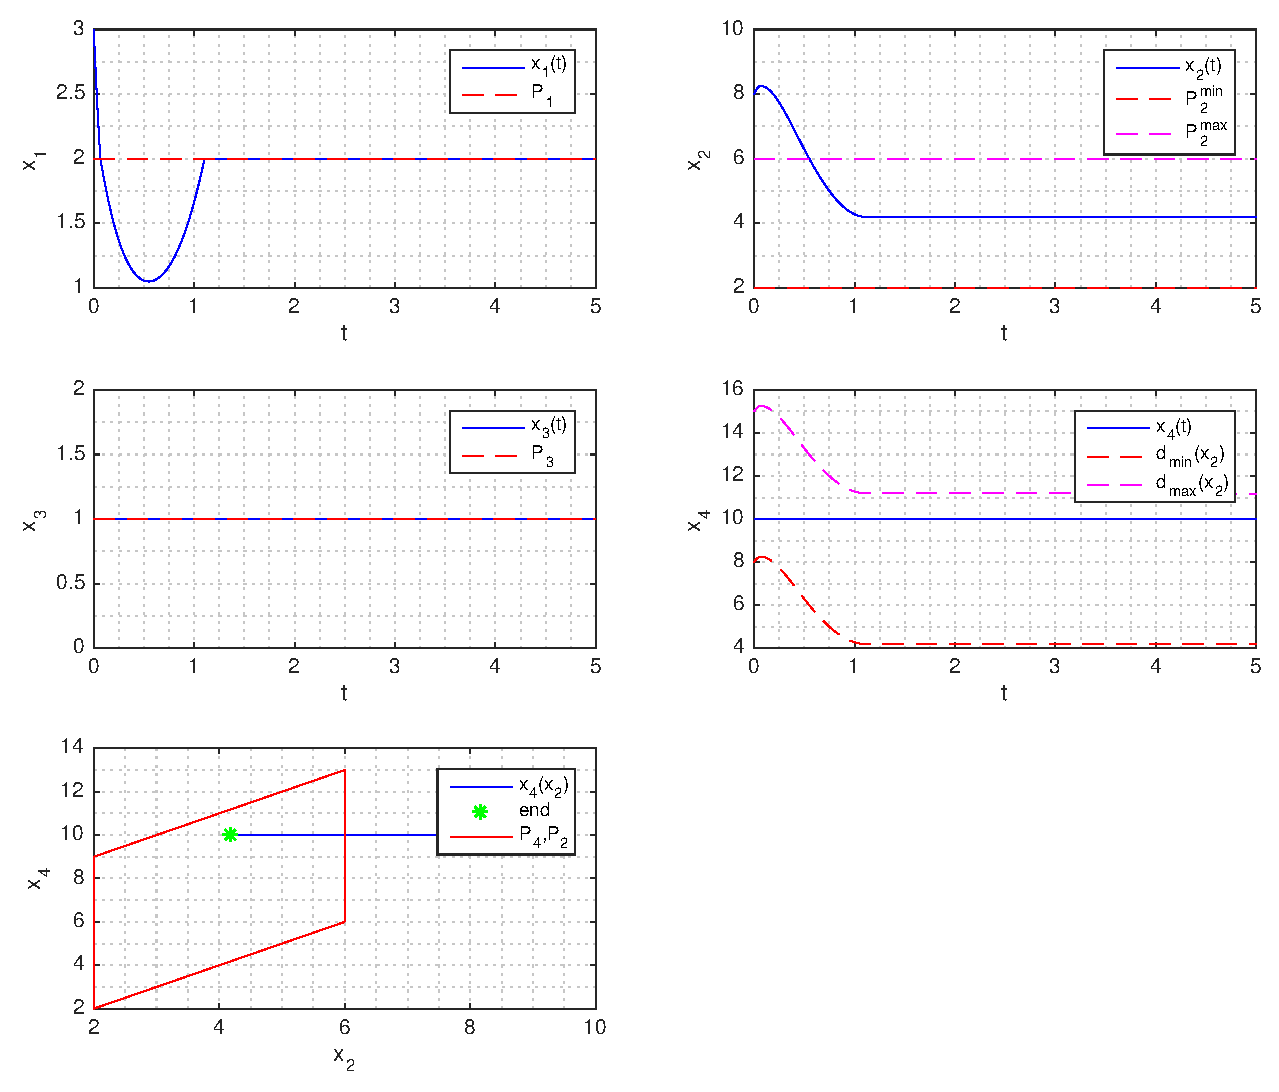
\includegraphics[width=0.7\textwidth]{x_3sl_total.eps}}
\caption{Скользящий режим по $x_3$.}
\end{figure}
%\FloatBarrier

% ------ Скользящий режим по х_1 -------
{\bf Скользящий режим по $x_1$.}

\beq
\left\{
\begin{aligned}
	x_1 &= P_1, \\
	\dot x_2 &= x_2(-r_2 - b_2x_3 + c_2P_1), \\
	\dot x_3 &= x_3(-r_3 + u_2 - b_3x_4 + c_3x_2), \\
	\dot x_4 &= x_4(-r_4 + c_4x_3), 
\end{aligned}
\right. \;\; \Leftrightarrow \;\;
\left\{
\begin{aligned}
	x_1 &= P_1, \\
	\dot x_2 &= b_2x_2(P_3 - x_3), \\
	\dot x_3 &= x_3(-r_3 + u_2 - b_3x_4 + c_3x_2), \\
	\dot x_4 &= c_4x_4(x_3 - P_3). 	
\end{aligned}
\label{system1}
\right.
\eeq

\begin{figure}[h]
\center{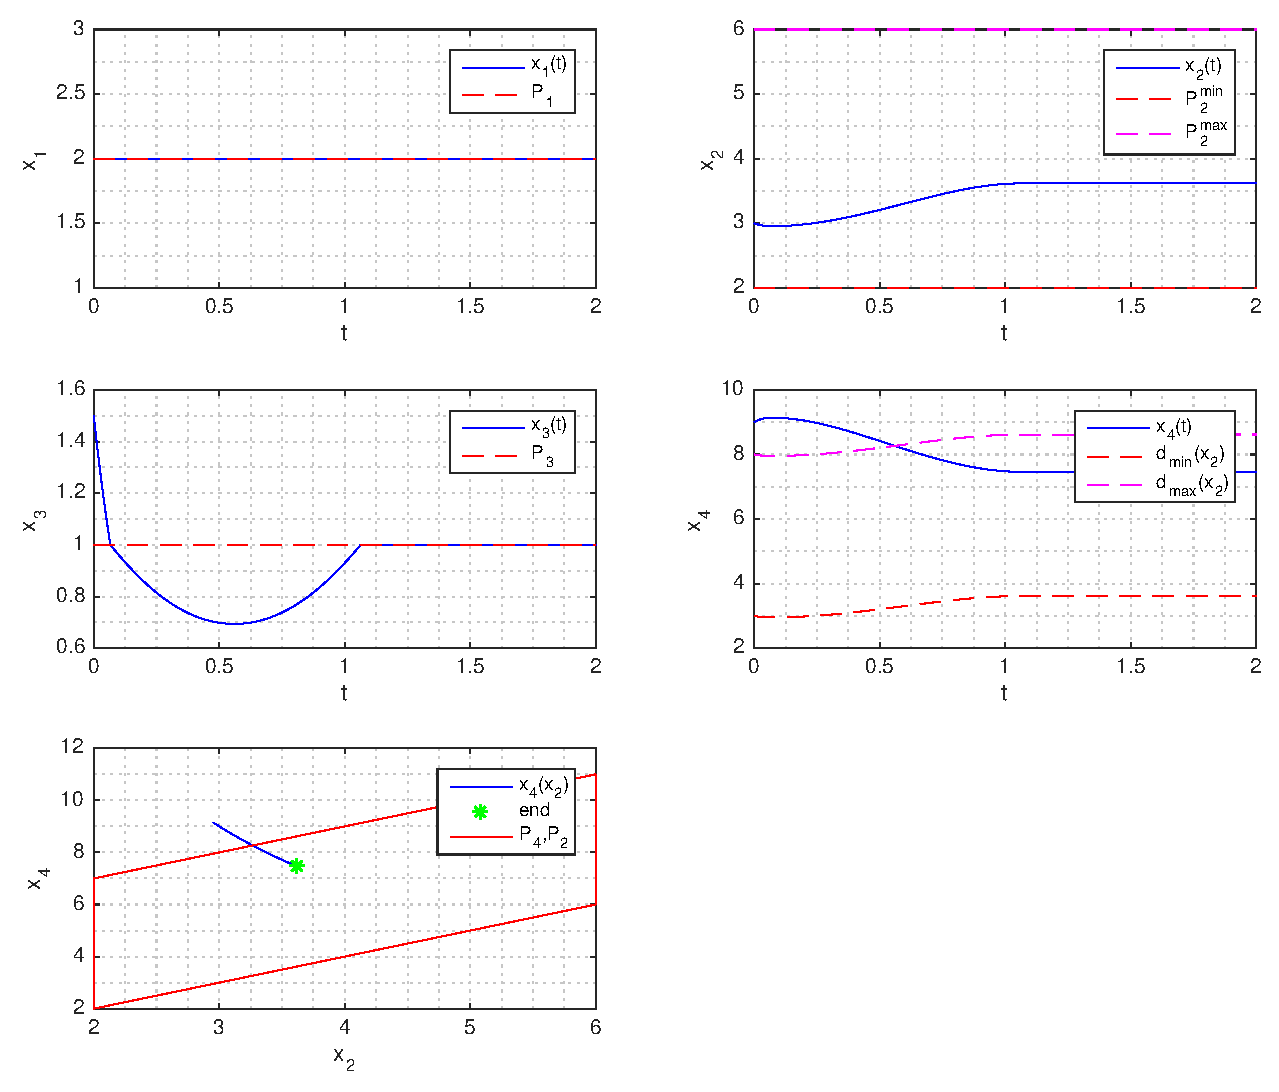
\includegraphics[width=0.7\textwidth]{x_1sl_total.eps}}
\caption{Скользящий режим по $x_1$.}
\end{figure}
%\FloatBarrier

Заметим, что $\text{sgn}(\dot x_4) = -\text{sgn}(\dot x_2) = \text{sgn}(x_3 - P_3).$ \\
Также заметим, что в случае $x_3 > P_3$ $$\text{sgn}(\dot x_3) =  \text{sgn}(x_4 - d_{min}(x_2)),$$ а в случае $x_3 < P_3$ $$\text{sgn}(\dot x_3) = \text{sgn}(x_4 -d_{max}(x_2)).$$

Таким образом будем рассматривать 4 случая в зависимости от знака $x_3 - P_3$ и $\dot x_3:$

% Тут наверное хорошо бы табличку

\begin{description}
	\item[Случай 1:] $x_3 > P_3, \; \dot x_3 > 0,$
	\item[Случай 2:] $x_3 > P_3, \; \dot x_3 < 0,$
	\item[Случай 3:] $x_3 < P_3, \; \dot x_3 > 0,$
	\item[Случай 4:] $x_3 < P_3, \; \dot x_3 < 0.$
\end{description}

Без ограничения общности будем считать, что скользящий режим по первой координате осуществляется с начального момента времени $t_0$.\\

\underline {\bf Случай 1.} 
$$x_3(t_0) > P_3, \; \dot x_3(t_0) > 0.$$
Из первого неравенства следует, что $\dot x_2(t_0) < 0, \dot x_4(t_0) > 0,$ а из второго --- что $x_4(t_0) < d_{min}(x_2).$

Таким образом $\dot x_3(t) > 0, \forall t : x_4(t) < d_{min}(x_2),$ поэтому, пока $x_4 < d_{min}(x_2)$, $ x_3 - P_3 \geqslant x_3(t_0) - P_3 = a_1 > 0.$ Тогда $\dot x_4 \geqslant c_4x_4(t_0)a_1, \dot x_2 < 0 \Rightarrow d_{min}(x_2) < d_{min}(x_2(t_0)),$ тогда мы можем оценить $t_1 \leqslant \frac{d_{min}(x_2(t_0)) - x_4(t_0)}{c_4x_4(t_0)a_1}$ --- время, за которое $x_4$ дойдет до $d_{min}(x_2)$.\\
Рассмотрим момент $t_1.$ \\
$\dot x_3(t_1) = 0,$ но $\ddot x_3(t_1) = \dot x_3(t_1)((-r_3 + u_2 - b_3x_4(t_1) + c_3x_2(t_1)) + x_3(t_1)(-b_3\dot x_4(t_1) + c_3 \dot x_2(t_1)) < 0,$ так что $\forall \Delta_1 > 0 \; \dot x_3(t_1 + \Delta_1) < 0,$ при этом $x_3(t_1 + \Delta_1) > P_3,$ так что теперь возникает случай 2.\\

\underline{\bf Случай 2.}
$$x_3(t_1) > P_3, \dot x_3(t_1) < 0.$$
Из первого неравенства следует, что $\dot x_2(t_1) < 0, \dot x_4(t_1) > 0,$ а из второго --- что $x_4(t_1) > d_{min}(x_2(t_1)).$ Докажем, что 
\begin{itemize}
	\item либо $\exists t_2 < \infty:  x_3(t_2) = P_3,$
	\item либо $\forall \varepsilon > 0 \: \exists t_2' : x_3(t) - P_3 < \varepsilon \; \forall t > t_2'.$
\end{itemize}
Предположим противное: $\forall t > t_1 \; x_3(t) > P_3 + \delta, \delta > 0.$ Тогда $\dot x_2(t) < b_2x_2\delta < 0,$ поэтому $\exists t_2^* : x_2(t_2^*) < P_2^{min},$ но тогда мы выходим из скользящего режима по первой координате, что выходит за рамки рассматриваемого случая.

Случай, когда $x_3$ попадает в $\varepsilon$-окрестность $P_3$ приводит нас в положение равновесия по всем координатам с точностью до бесконечно малой величины.

Если же $\exists t_2 : x_3(t_2) = P_3,$ то в зависимости от того, где в этот момент находится четвертая координата, мы либо решили задачу, либо переходим к случаю 4:
\begin{itemize}
	\item $x_4(t_2) \in [d_{min}(x_2(t_2)), d_{max}(x_2(t_2))], \; x_3(t_2) = P_3, \; x_2(t_2) \in [P_2^{min}, P_2^{max}], \; x_1(t_2) = P_1 \Rightarrow x(t_2) = P(u).$
	\item $x_4(t_2) > d_{max}(x_2(t_2)) \Rightarrow \dot x_3(t_2) < 0, \; \forall \Delta_2 > 0 \; x_3(t_2 + \Delta_2) < P_3 \Rightarrow$ переходим к случаю 4, заменив $t_2 + \Delta_2$ на $t_2$.
\end{itemize}

\underline{\bf Случай 4.}
$$x_3(t_2) < P_3, \dot x_3(t_2) < 0.$$
Из первого неравенства следует, что $\dot x_2(t_2) > 0, \dot x_4(t_2) < 0,$ а из второго --- что $x_4(t_2) > d_{max}(x_2(t_2)).$

Аналогично случаю 1 $\dot x_3(t) < 0, \forall t : x_4(t) > d_{max}(x_2),$ поэтому, пока $x_4 > d_{max}(x_2)$, $ x_3 - P_3\leqslant x_3(t_2) - P_3 = a_2 < 0.$ Тогда $\dot x_4 \leqslant -c_4x_4(t_2)a_2, \dot x_2 > 0 \Rightarrow d_{max}(x_2) > d_{max}(x_2(t_2)),$ тогда $\exists t_3 : x_4(t_3) = d_{max}(x_2).$ \\
Рассмотрим момент $t_3.$ \\
$\dot x_3(t_3) = 0,$ но $\ddot x_3(t_3) = \dot x_3(t_3)((-r_3 + u_2 - b_3x_4(t_3) + c_3x_2(t_3)) + x_3(t_3)(-b_3\dot x_4(t_3) + c_3 \dot x_2(t_3)) > 0,$ так что $\forall \Delta_3 > 0 \; \dot x_3(t_3 + \Delta_3) > 0,$ при этом $x_3(t_3 + \Delta_3) < P_3,$ так что теперь возникает случай 3.\\

\underline{\bf Случай 3.}
$$x_3(t_3) < P_3, \dot x_3(t_3) > 0.$$
Из первого неравенства следует, что $\dot x_2(t_3) > 0, \dot x_4(t_3) < 0,$ а из второго --- что $x_4(t_3) < d_{max}(x_2(t_3)).$

Как и в случае 2, мы можем доказать, что 
\begin{itemize}
	\item либо $\exists t_4 < \infty:  x_3(t_4) = P_3,$
	\item либо $\forall \varepsilon > 0 \: \exists t_4' : x_3(t) - P_3 < \varepsilon, \forall t > t_4'.$
\end{itemize}

Однако в данном случае реализуется только первый пункт, то есть всегда существует конечный момент времени, в который $x_3 = P_3.$ Докажем невозможность второго пункта. Рассмотрим $\ddot x_3(t), \; t > t_3.$
$$\ddot x_3(t) = \dot x_3(t)((-r_3 + u_2 - b_3x_4(t) + c_3x_2(t)) + x_3(t)(-b_3\dot x_4(t) + c_3 \dot x_2(t)) > 0 \; \forall t : x_3(t) < P_3, $$ 
так как $\dot x_3(t)((-r_3 + u_2 - b_3x_4(t) + c_3x_2(t)) \geqslant 0 \; \forall t, \; x_3(t) > 0 \; \forall t, \; \dot x_4(t) < 0, \dot x_2(t) > 0 \; \forall t : x_3(t) < P_3.$
Таким образом невозможно асимптотическое приближение к положению равновесия, как в случае 2. Но как и в случае 2, дальнейшая динамика системы зависит от $x_4(t_4):$

\begin{itemize}
	\item Если $x_4(t_4) \in [d_{min}(x_2(t_4)), d_{max}(x_2(t_4))], \; x_3(t_4) = P_3, \; x_2(t_4) \in [P_2^{min}, P_2^{max}], \; x_1(t_4) = P_1 \Rightarrow x(t_4) = P(u).$
	\item Если $x_4(t_4) < d_{min}(x_2(t_4)) \Rightarrow \dot x_3(t_4) > 0, \; \forall \Delta_4 > 0 \; x_3(t_4 + \Delta_4) > P_3 \Rightarrow$ переходим к случаю 1, заменив $t_4 + \Delta_4$ на $t_0$.
\end{itemize}

Таким образом схематично мы можем изобразить, как один случай сводится к другому, на следующей диаграмме, где состояние F означает решение задачи попадания точно во множество положений равновесия, а $\varepsilon$ --- попадание в $\varepsilon$-окрестность положения равновесия:

\[
\begin{diagram}
\node{1} \arrow[4]{e}{}
\node[4]{2} \arrow[3]{s}{} \arrow[1]{wsw} \arrow[2]{sw}\\
\node[3]{\varepsilon}\\
\node[3]{F}\\
\node{3} \arrow[3]{n}{} \arrow[1]{ene} 
\node[4]{4} \arrow[4]{w}
\end{diagram}
\]

\begin{figure}[h]
\center{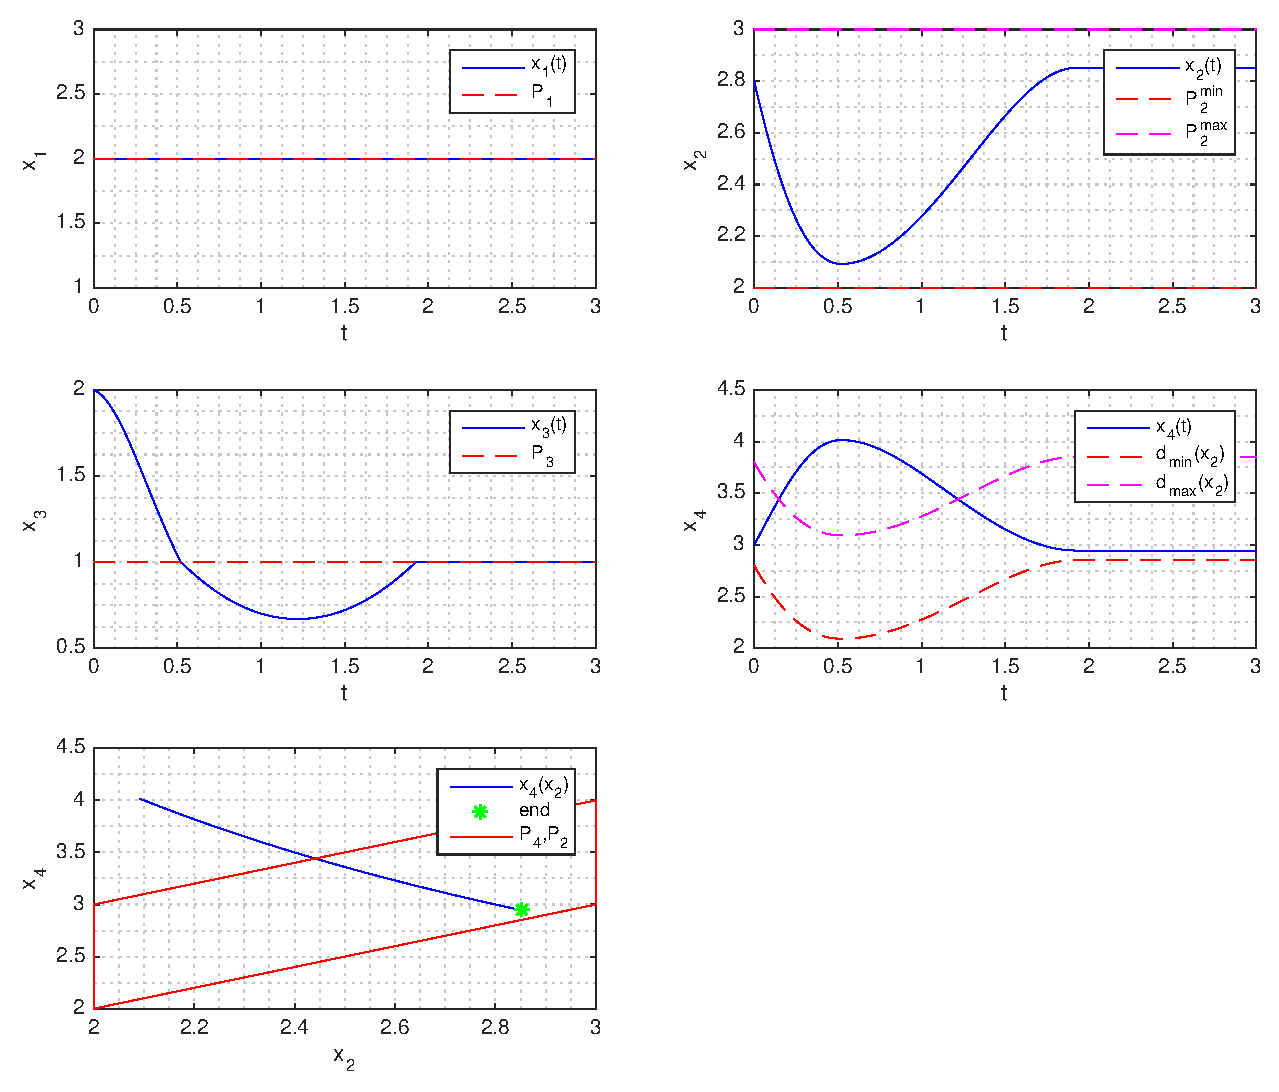
\includegraphics[width=0.6\textwidth]{2_4_3_F.eps}}
\caption{Реализация случаев 2 $\to$ 4 $\to$ 3 $\to$ F.}
\end{figure}
\FloatBarrier

\section{Заключение}

Данная работа представляет собой первый этап в рассмотрении четырехмерной пищевой цепи, в которой управляющие параметры входят в показатели роста и смертности первого и третьего вида. Предложен метод синтеза управления для задачи попадания в произвольно малую $\varepsilon$-окрестность положения равновесия. Доказано, что такой синтез позволяет решить задачу за конечное время. Также исследовано поведение системы в скользящих режимах. 

Дальнейшее рассмотрение задачи предполагает изучение возможности попадания в точности в положение равновесия за конечное время. Численные эксперименты позволяют предположить, что таковая возможность есть, но требует более тонкого анализа, который выходит за пределы представленной работы. Ниже представлен график зависимости времени достижения $\varepsilon$-окрестности от ее размеров в логарифмическом масштабе по оси $x$. Из него видно, что с уменьшением окрестности время увеличивается незначительно.

\begin{figure}[bh]
\center{\includegraphics[width=0.6\textwidth]{time_eps.eps}}
\caption{Зависимость времени достижения $\varepsilon$-окрестности от ее размеров.}
\end{figure}
\FloatBarrier

%===========Библиография============
\clearpage
\newpage
\begin{thebibliography}{0}

	\bibitem{Lotka} {\it Lotka A. J.} Analytical Note on Certain Rhythmic Relations in Organic Systems // Proc. Natl. Acad. Sci. U.S. 1920. V. 6, P. 410-415.
	
	\bibitem{Murray} {\it Murray~J.~D.} Mathematical Biology. Springer. 2002.
	
	\bibitem{Basykin} {\it Базыкин~А.~Д.} Математическая биофизика взаимодействующих популяций. М.: Наука. 1985.
	
	\bibitem{Ruble} {\it Рублев~И.~В., Простяков~П.~В.} Построение множества достижимости системы Лотка--Вольтерра. Общий случай. // 2018 (подготовлена к публикации).
	
	\bibitem{three_spec} {\it Sze-Bi~Hsu, Shigui~Ruan, Ting-Hui~Yang} Analysis of three species Lotka–Volterra food web models with omnivory // Journal of Mathematical Analysis and Applications. 2015. V. 426. P. 659--687
	
	\bibitem{darboux} {\it Laurent Cairo} Darboux First Integral Conditions and Integrability of the 3D Lotka-Volterra System // Journal of Nonlinear Mathematical Physics. 2000, V. 7, N 4. P. 511--531.
   
    	\bibitem{MathBio} {\it Massarelli~N., Hoffman~K., Previte~J.~P.} Effect of parity on productivity and sustainability of Lotka–Volterra food chains. // Mathematical Biology. December of 2014. V. 69. P. 1609--1626.
	
	\bibitem{Lyapunov} {\it Ляпунов~А.~М.} Общая задача об устойчивости движения. Москва. Государственное издательство технико-теоретической литературы. 1950.
    
    	\bibitem{Filippov} {\it Филиппов~А.~Ф.} Дифференциальные уравнения с разрывной правой частью. М.: Наука. 1985.
	   
    	\bibitem{Bratus} {\it Братусь~A.~C., Новожилов~А.~С., Платонов~А.~П.} Динамические модели и модели биологии. М.: Физматлит, 2010.
	 
	 \bibitem{Vasiliev} {\it Ф.П.Васьльев} Методы оптимизации. Москва. Факториал пресс. 2012. с. 176.

	 \bibitem{Aushkap} {\it Н.~С.~Аушкап} Задача достижимости для модели межвидового взаимодействия // Дипломная работа. Кафедра системного анализа факультета ВМК МГУ. 2013
	 
\end{thebibliography}
   
\end{document}